\begin{doublespace}

For the user interface design shown in this chapter, we were influenced by the previous gear design application and SolidWorks. The point of having this new interface redesign was to have the user be able to visualize what they were creating and give them an organized interface that that allowed them to edit gear properties with ease. Some of the changes made in constructing this design were to have a 3D viewer, which gave the user a visualization, and to remove repeating inputs that led to a messy screen.

The user interface of the gear box application is split into five major parts: the menu, the top bar, the left bar, the 3D view, and the other pop-up windows. The menu contains settings and toggles for certain options. The top bar is for important actions, such as generating the design in SolidWorks. The left bar is for navigating and editing the gear train and its properties. The 3D view is to visualize the gear train and the edits made. The rest of the pop-up screens are for analysis and detailed gear train editing.

\subsection{Main Menu}

The main menu consists of the application title and two drop downs located at the top of the screen (see Figure~\ref{fig:firstopen}). One drop down contains ``File'' and the other contains ``Options''. File has content relating to the actions regarding the application files, such as opening or saving a gear train design (Figure~\ref{fig:menufile}). Options contains application settings (Figure~\ref{fig:menuOptions}).

\begin{figure}[htbp]
    \centering
    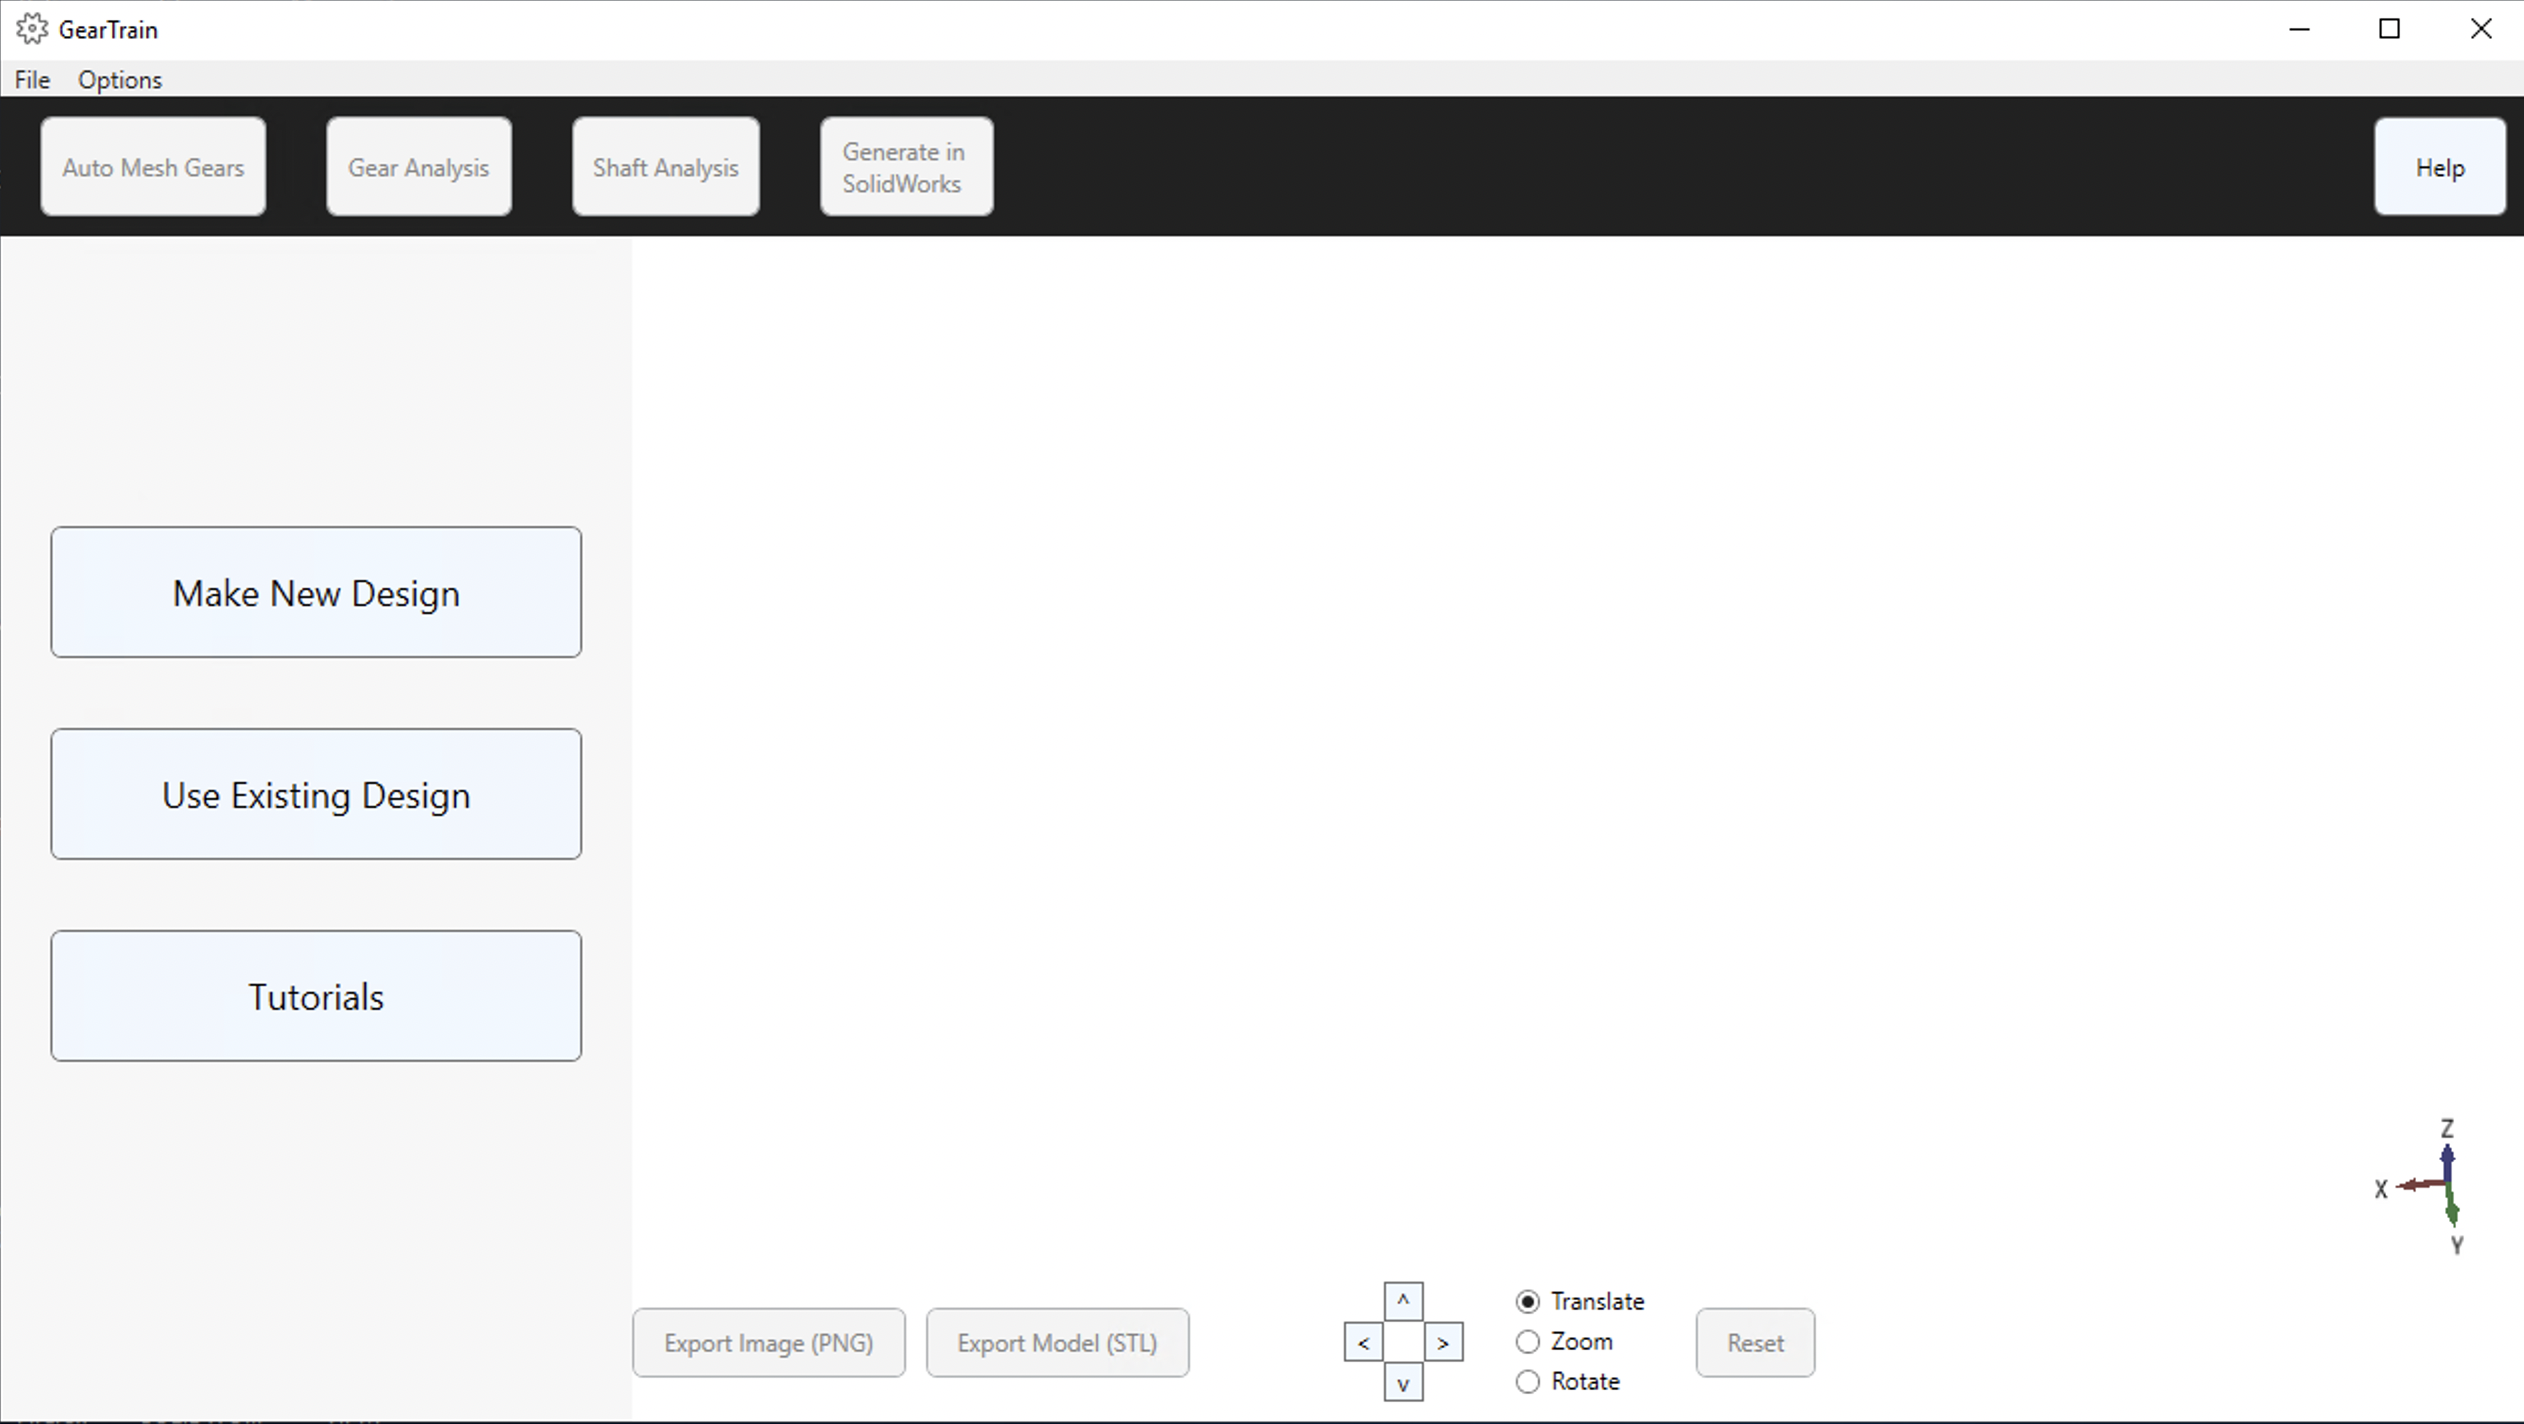
\includegraphics[width=1\textwidth]{full_app_first_opened}
    \caption{Interface when the application is first opened (start screen).}
    \label{fig:firstopen}
\end{figure}

\subsubsection{File Drop-down}

We added a File drop-down menu (as seen in Figure~\ref{fig:menufile}) to the main menu to access file-related actions. The first item, ``Open'', is for opening an existing gear train. It is then followed by ``New'' which is for starting a new gear train design. The ``Save'' item is for saving the current gear train being worked on. There is also ``Open Output Directory,'' which will open the output directory in the file explorer. The output directory is where files that are created by SolidWorks are placed during the generation process. These files include SolidWorks part (SLDPRT) files for each gear train component, as well as the completed assembly (SLDASM). Finally, there is ``Exit,'' which closes GearTrain and does not save (but prompts the user if they would like to save first).

\begin{figure}[htbp]
    \centering
    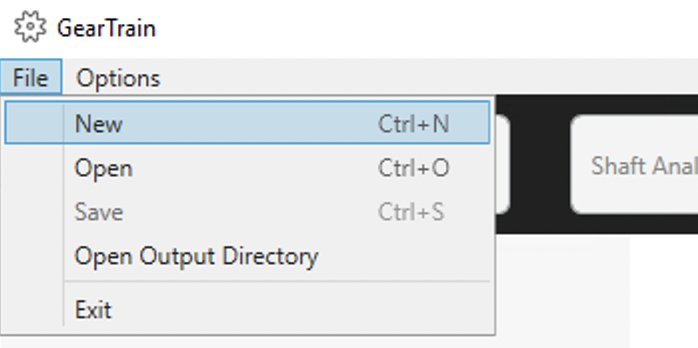
\includegraphics[width=.6\textwidth]{app_menu_file}
    \caption{Menu - File drop down.}
    \label{fig:menufile}
\end{figure}

\subsubsection{Options Drop-down}

The options drop-down contains settings for the application, as well as options for the SolidWorks generation (Figure~\ref{fig:menuOptions}). The drop-down splits into two other drop-downs and an action. The first one drop-down being ``Units'', which shows two options. One of them is for metric and the other for imperial. The second drop-down, ``Generation Settings'', contains toggles related to settings used when the user generates the gear train. This includes Creating Parts, Creating an Assembly, Creating Bearings, Generating in Background (creates a background task that is not visible to the user and may use less resources), and Auto Generating Shafts. These settings affect the design generated in SolidWorks. The last item, ``Set Output Directory,'' allows the user to choose where 3D files are put when the gear train is generated in SolidWorks.

\begin{figure}[htbp]
    \centering
    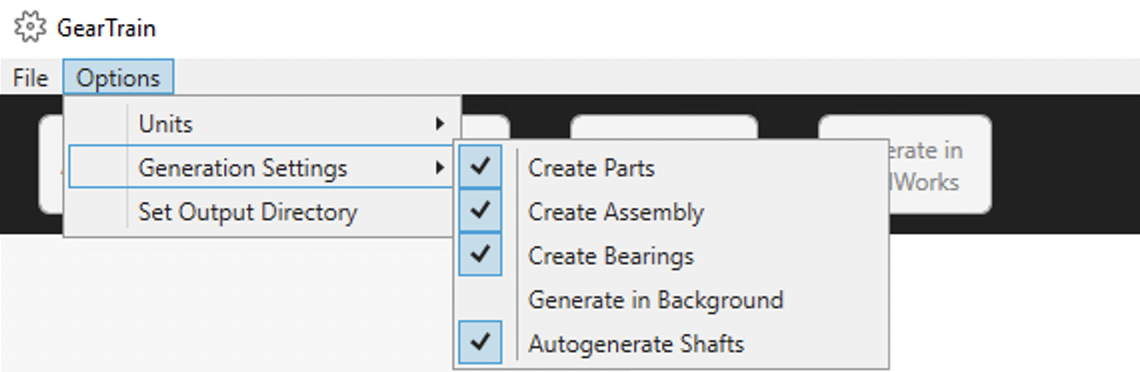
\includegraphics[width=.8\textwidth]{app_menu_options}
    \caption{Menu - Options drop down.}
    \label{fig:menuOptions}
\end{figure}

\subsection{Top Bar}

Figure~\ref{fig:topbar} shows the top bar, which is located at the top of the application screen just under the main menu (see Figure~\ref{fig:firstopen}). We decided to have it here since it would not get in the way of the other parts of the application such as the left bar and the 3D view. It contains a series of buttons from left to right in order of importance. We defined their order by how essential their actions are to the application and how often they might be pressed. These buttons contain actions that can be used when a gear train is being designed.

The buttons contain the Auto Mesh function (which adjusts gear positions so they are touching properly), the Gear/Shaft Analysis windows, the Generation function (sends the design to SolidWorks to be generated), and the Help button (opens the help website in the user's default browser. We selected these actions because they would have to be able to run at anytime a gear train is open. To make sure they are not used until a gear train design is open, the buttons are grayed-out and disabled when the application is first opened.

\begin{figure}[htbp]
    \centering
    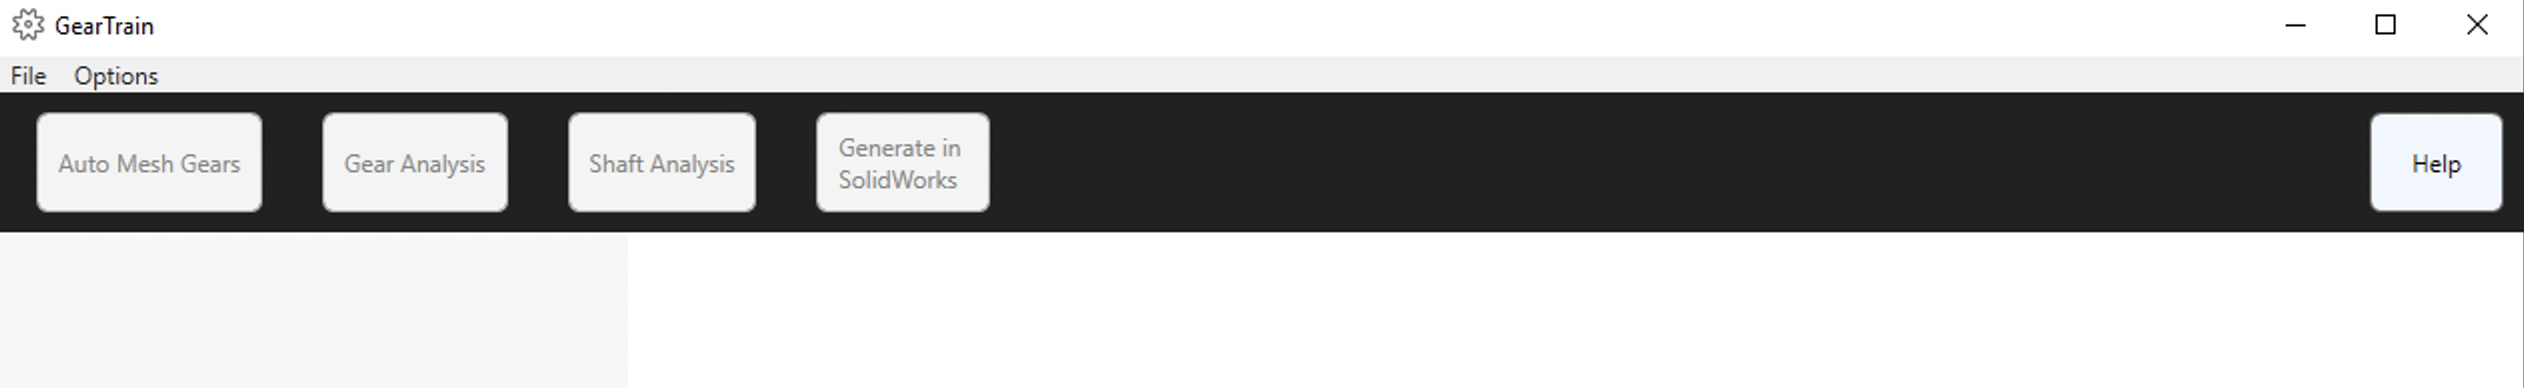
\includegraphics[width=1\textwidth]{app_top_bar}
    \caption{App top bar.}
    \label{fig:topbar}
\end{figure}

\subsection{Left Bar}

The left bar is at the left most side of the application. It contains various screens during different states of the application. For example, when the application is first opened the start screen is shown in the left bar. Then, depending on the user selection, the screens will change or be propagated with new data.

\subsubsection{Start Screen}

The left bar shows the start screen when the application first opens (Figure~\ref{fig:firstopen}). This displays three especially big, stacked buttons for the user to start with. The buttons are ``Use Existing Design'' (opens an existing gear train from a file), ``Make New Design'' (creates a new gear train design), and ``Tutorials'' (opens the Help website in the user's default browser). These highlight the main actions a user might do when they first open the application. We decided on having the help information outside the application since a user might want to look at help while they do not have the application open. The information could also contain videos, which are more easily implemented on a website. 

\subsubsection{Gear Sets Screen}

Figure~\ref{fig:leftgearsets} shows the Gear Sets screen, which shows a list of all the gear sets in the current gear train. They are listed and numbered from top to bottom. There are also action buttons to be applied to the gear sets listed right above. These include a button for adding a new gear set, editing a gear set, and deleting a gear set. The ``Edit'' button navigates the left bar to the edit gear set screen, while the ``Add'' and ``Delete'' buttons simply change the contents of the list. At the bottom, there is a ``Back'' button. It will prompt the user to save their current design before returning to the start screen.

\begin{figure}[htbp]
    \centering
    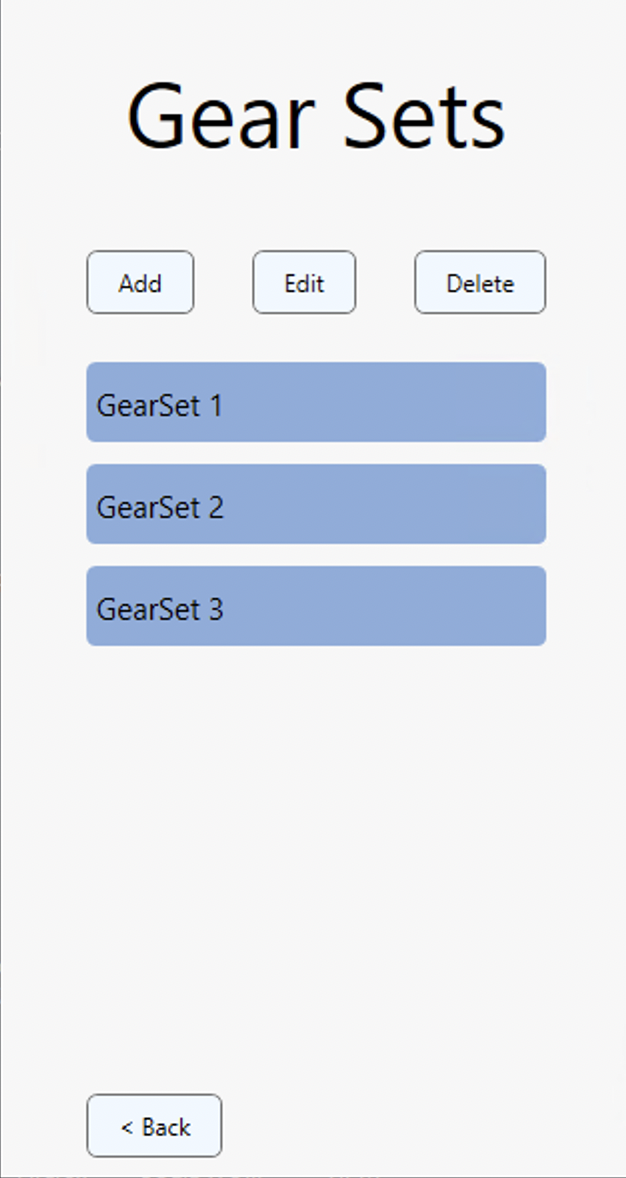
\includegraphics[width=.5\textwidth,]{gearsets}
    \caption{Left bar - Gear Sets screen.}
    \label{fig:leftgearsets}
\end{figure}

\subsubsection{Edit Gear Set Screen}

Figure~\ref{fig:lefteditgearset} shows the edit gear screen. This screen allows editing the properties of a specific gear set in a gear train. The name of the gear set is displayed at the very top. It is then followed by a combo-box or a drop-down containing the different gear types that a user can choose. Below is the list of gears in the gear set and buttons with actions that can be applied to the list. One action is to add an idler gear and the other is to edit the shaft alignment in regards to a a gear. When a gear is selected from the list, a smaller area below appears with its respective properties. All of the properties can be edited under a combo-box or text-box. There are also back and revert buttons. All changes made in this screen are automatically saved. The user can choose to revert changes made to when the edit gear set screen first loaded. The back button will ask the user if they want to keep the changes they made before going back to the gear sets screen.

\begin{figure}[htbp]
    \centering
    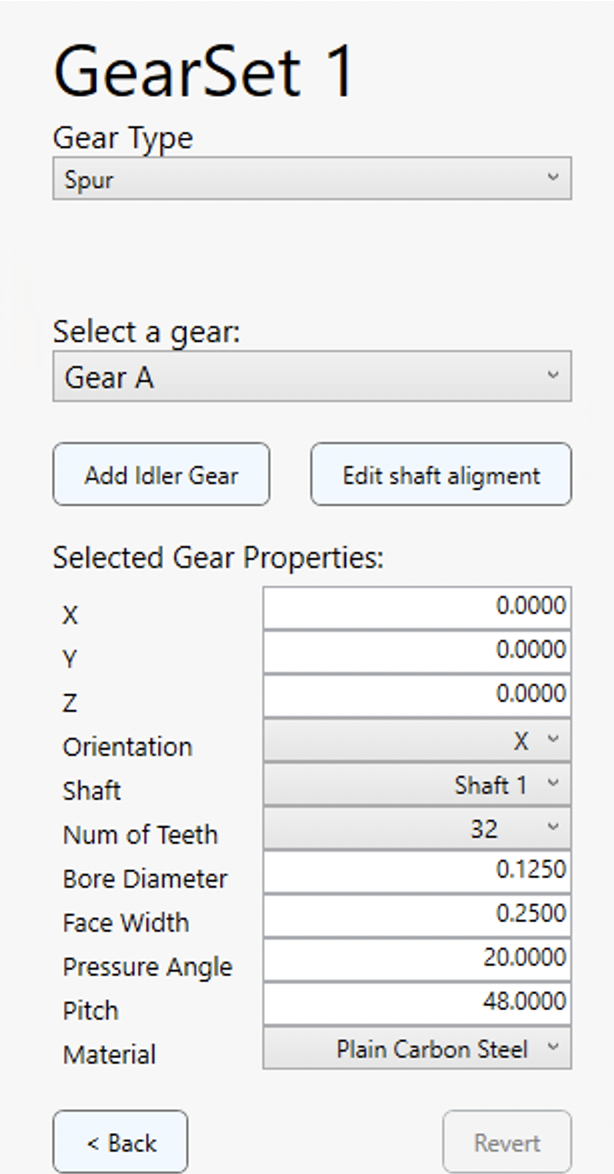
\includegraphics[width=.5\textwidth]{app_left_bar_gear_set_edit}
    \caption{Left bar - Edit Gear Set screen.}
    \label{fig:lefteditgearset}
\end{figure}

\subsection{3D View}

Figure~\ref{fig:3dex} shows the 3D viewer, which is a screen where the 3D representation of the gear train is displayed. It is located on the bottom right of the screen, but takes up a majority of the window, using the same height as the left bar. The 3D view, as the name suggests, contains a 3D representation of the gear train that updates as the user makes changes to it. There is a coordinate system on the bottom right corner of the 3D viewer to let the user know the orientation of the 3D model. Below the viewer, there are controls to manipulate the camera, such as rotate, pan, and zoom. There are two export buttons that allow the user to save the contents of the 3D viewer as a PNG or STL file.

\begin{figure}[htbp]
    \centering
    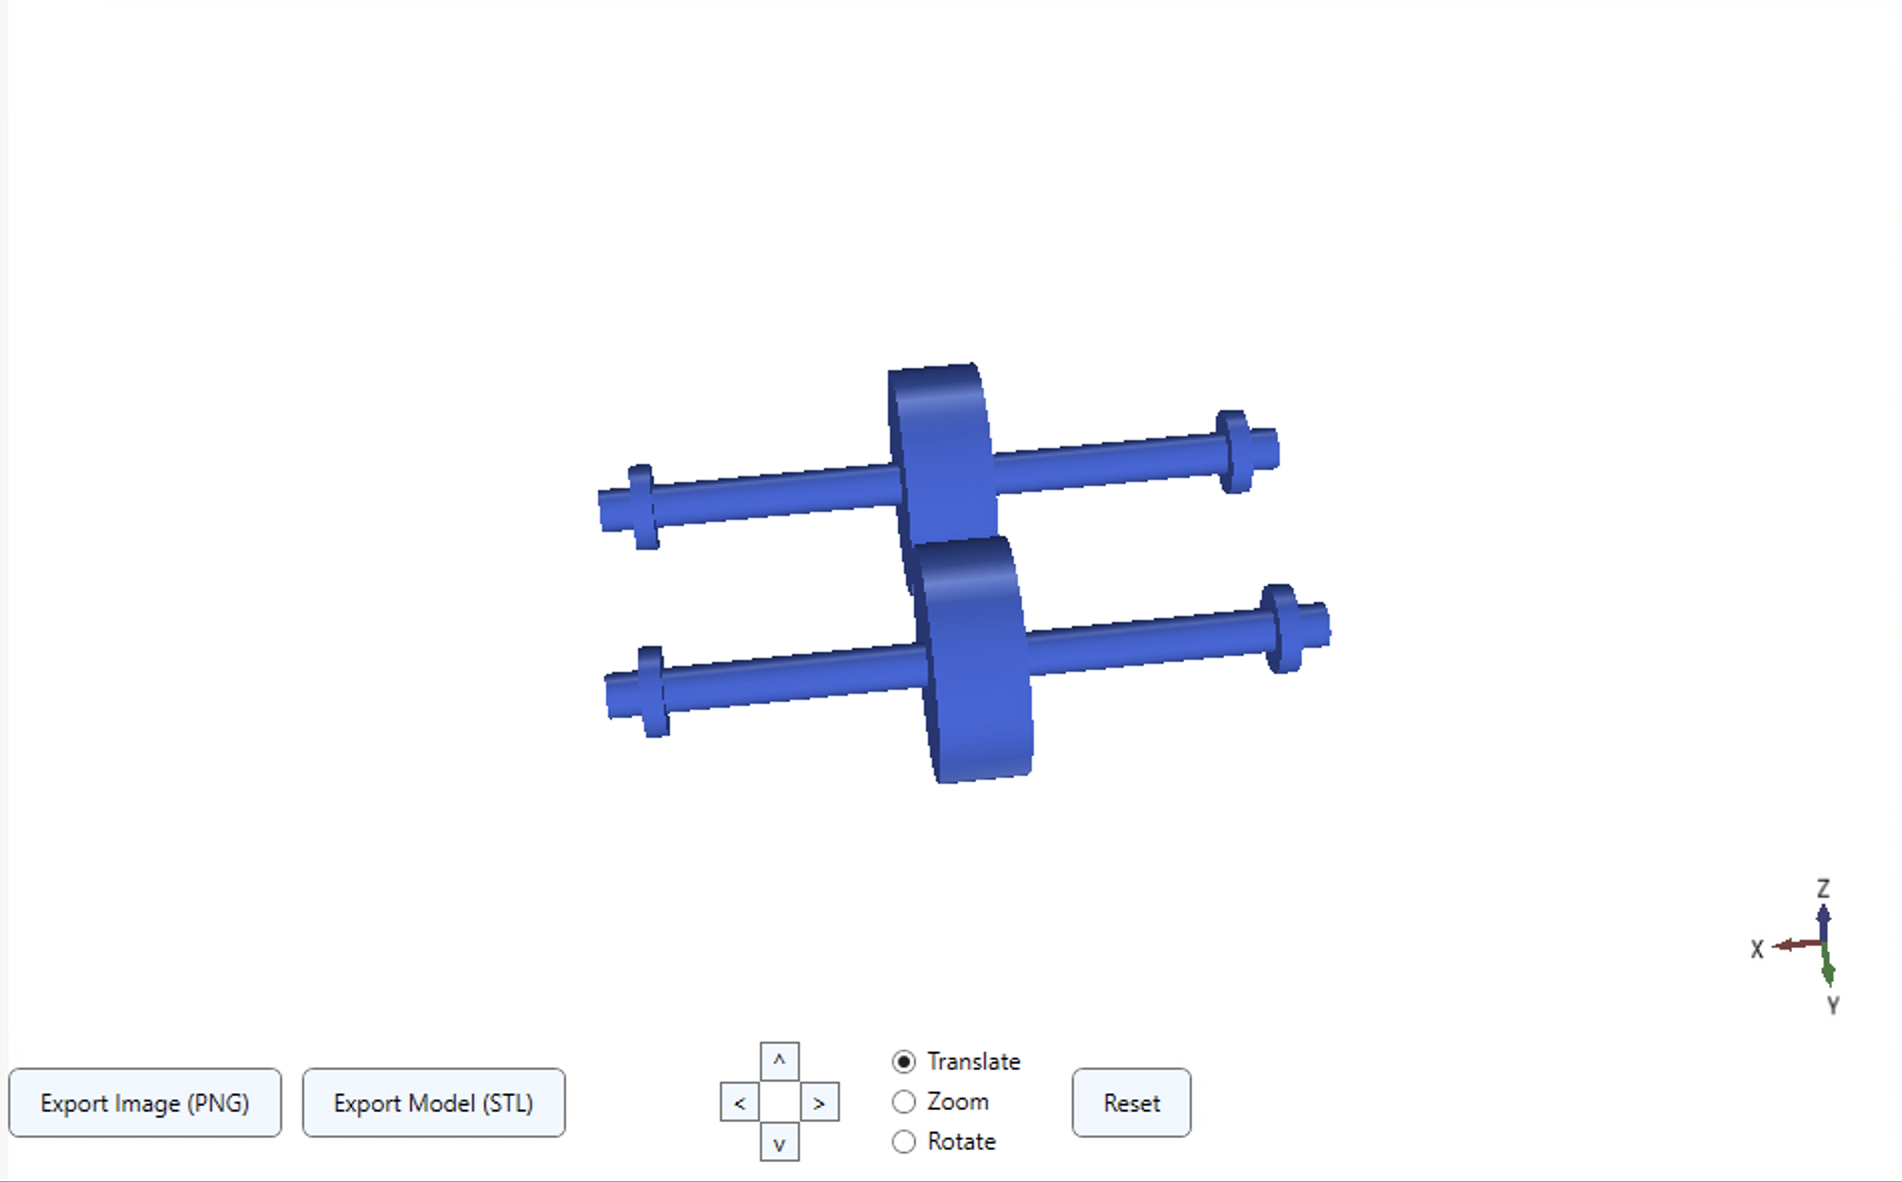
\includegraphics[width=.9\textwidth]{3dExample}
    \caption{3D viewer displaying a static simple representation of a gear set.}
    \label{fig:3dex}
\end{figure}

\subsection{Other Interfaces}

\subsubsection{Edit Shaft Window}

Figure~\ref{fig:editshaft} shows the edit shaft window, which can be navigated to from the edit gear set screen by clicking on the ``Edit Shaft Alignment'' button as seen in Figure~\ref{fig:lefteditgearset}. The Edit Shaft screen has a 2D representation of a shaft and the gears and bearings connected to it. There is also a bar on the side to edit alignment properties like the length of the shaft and the positions of the items on the shaft. The values will be editable through text boxes, but the gears and bearings on the shaft can also be dragged along the shaft by clicking and holding the mouse.

\begin{figure}[htbp]
    \centering
    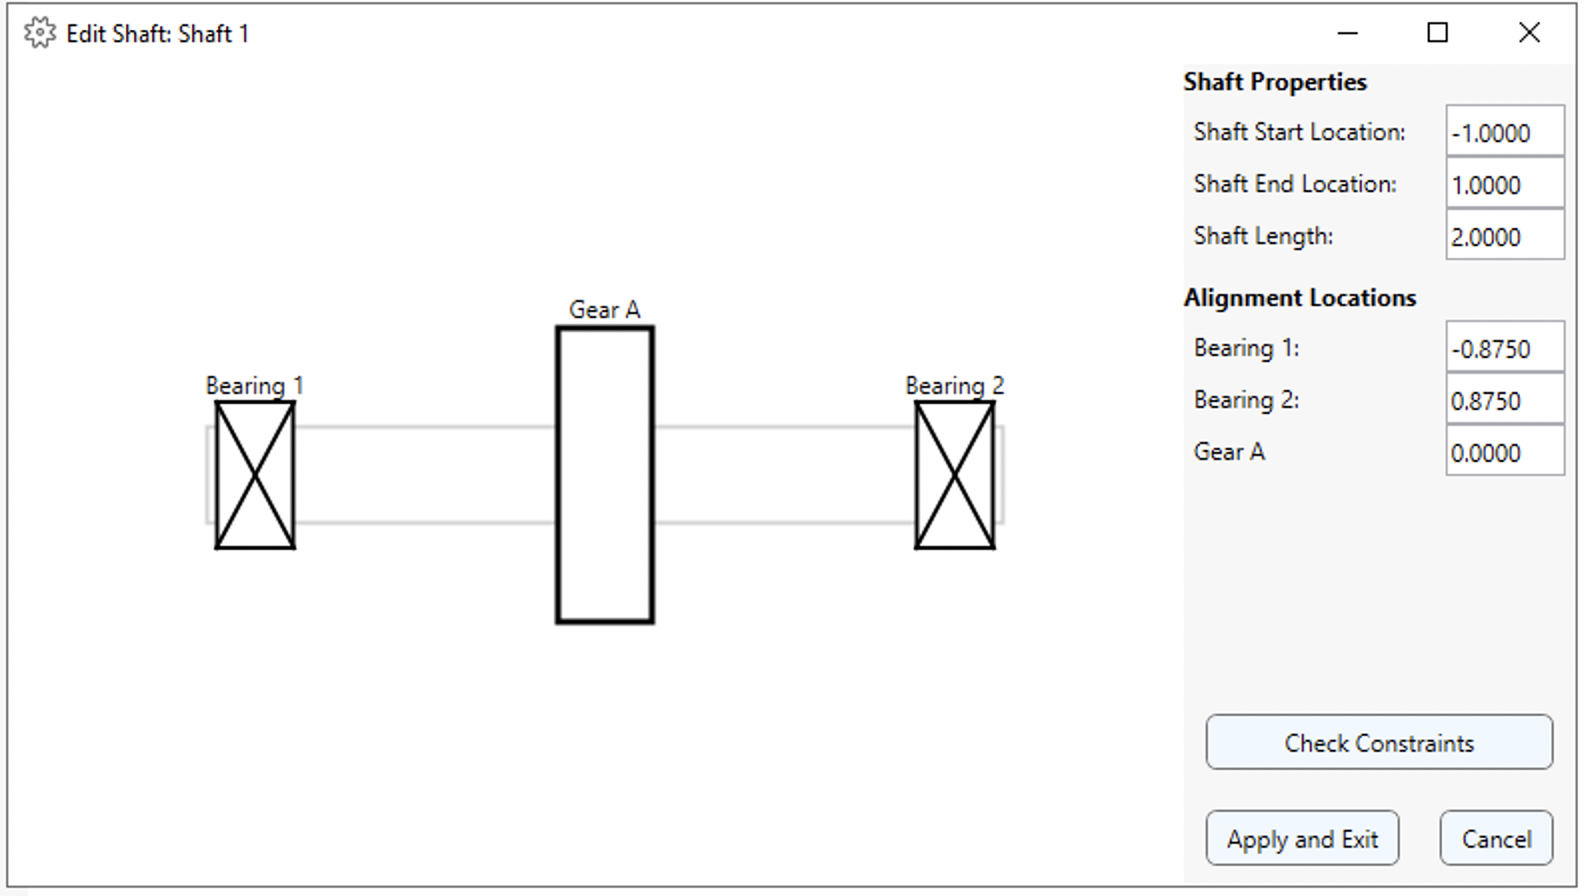
\includegraphics[width=.8\textwidth]{edit-shaft}
    \caption{Edit Shaft window.}
    \label{fig:editshaft}
\end{figure}

\subsubsection{Gear Analysis}

Figure~\ref{fig:gearanaly} shows the gear analysis window. The interface for the Analyze Gear and Shaft windows are not final, and they may not be final for this iteration of the project since the gear analysis code has not been integrated (see Chapter~\ref{sec:concl}). They are for making stress analyses on gears and shaft. There is an initial screen to input information relating to the gear or shaft. Once the user selects the analyze button, the application will navigate to a separate screen where the analyses that have been made are shown. The user is only shown some of the most commonly used analysis data points, but they are given the option to save the full analysis result to a CSV (comma-separated values) file.

\begin{figure}[H]
    \centering
    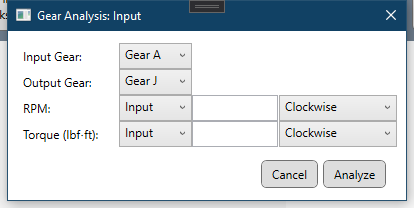
\includegraphics[width=0.8\textwidth]{gearanaly}
    \caption{Gear analysis screen.}
    \label{fig:gearanaly}
\end{figure}

\end{doublespace}